\documentclass[12pt,aspectratio=169]{beamer}

\usepackage[utf8]{inputenc}
\usepackage[T1]{fontenc}
\usepackage{mathabx}
\usepackage{mathpazo}
\usepackage{eulervm}
\usepackage{natbib}
\usepackage{siunitx}

%% Load the markdown package
\usepackage[citations,footnotes,definitionLists,hashEnumerators,smartEllipses,tightLists=false,pipeTables,tableCaptions,hybrid]{markdown}
%%begin novalidate
\markdownSetup{rendererPrototypes={
 link = {\href{#2}{#1}},
 headingOne = {\section{#1}},
 headingTwo = {\subsection{#1}},
 headingThree = {\begin{frame}\frametitle{#1}},
 headingFour = {\begin{block}{#1}},
 horizontalRule = {\end{block}}
}}
%%end novalidate

\usetheme{AWI}
\usepackage{appendixnumberbeamer}
\usepackage{amsmath}
\usepackage{booktabs}
\usepackage[scale=2]{ccicons}
\usepackage{tikz}
\usetikzlibrary{calc}
\usepackage{pgfplots}
\usepgfplotslibrary{dateplot}
\usepackage{xspace}

\usetheme[progressbar=frametitle]{metropolis}

\definecolor{red}{RGB}{182,15,15}     % extra dark to distinguish from green
\definecolor{yellow}{RGB}{230,195,22} % 
\definecolor{blue}{RGB}{0,116,186}
\definecolor{green}{RGB}{75,185,45}   % extra light
% AWI and Helmholtz
\definecolor{Helmholtzblau}{RGB}{0,90,160}
\definecolor{Helmholtzgruen}{RGB}{140,180,35}
\definecolor{Helmholtzdblau}{RGB}{10,45,110} % sekundär Farbe
\definecolor{Helmholtzgrau}{RGB}{90,105,110} % sekundär Farbe
\definecolor{Helmholtztuerkis}{RGB}{50,100,105} % Bereich Erde und Umwelt
\definecolor{AWIblau}{RGB}{0,172,229}
\definecolor{AWIdblau}{RGB}{0,62,110} % sekundär Farbe
\definecolor{AWIgrau}{RGB}{188,189,191} % sekundär Farbe
\definecolor{AWIdgrau}{RGB}{75,75,75} % sekundär Farbe
\definecolor{background}{RGB}{255,255,255}

%Adjust color theme
\setbeamercolor{background canvas}{bg=background}
\setbeamercolor{frametitle}{bg=background}
\setbeamercolor{title separator}{fg=AWIblau}
\setbeamercolor{footline}{fg=AWIgrau}
\setbeamercolor{progress bar}{fg=AWIblau, bg=AWIgrau}

\DeclareMathOperator{\sgn}{sgn}
\newcommand{\R}{\mathbb{R}}
\newcommand{\E}{\mathbb{E}}
\newcommand{\eye}{\mathbb{I}}
\newcommand{\mbf}[1]{\mathbf{#1}}
\newcommand{\T}{\intercal}
\newcommand{\norm}[1]{\left\lVert{#1}\right\rVert}

\unitlength=1cm

\title{A gentle introduction to Bayesian statistics and modeling - Part I}
\author{Brian Groenke}
\date{July 2024}

\begin{document}
\maketitle
\addtocounter{framenumber}{-1}

\AtBeginSection[]
{
    \begin{frame}
        \frametitle{Table of Contents}
        \tableofcontents[currentsection]
    \end{frame}
}

\section{Part I: A Tale of Two Statisticians}

\begin{frame}{Probability according to Cicero}
    \centering
    \textit{``That is probable which for the most part usually comes to pass, or which is a part of the ordinary beliefs of mankind or which contains in itself some resemblance to these qualities, whether such resemblance be true or false.''}
    - Cicero, ca. 80 BCE
\end{frame}

\begin{frame}{The Frequentist vs. The Bayesian}
    \textbf{The Frequentist} argues that probability is strictly defined by the \textit{frequency} of an event over an \textit{infinite} number of samples or experiments.
    \pause\newline
    
    \textbf{The Bayesian} argues that probability quantifies our \textbf{uncertainty} about a prediction, parameter, or hypothesis.
    \pause\newline
    
    For the Frequentist, the "true" (population) parameters are fixed while the observed data (samples) are random.
    \pause\newline
    
    For the Bayesian, all variables are random variables, including the parameters!
\end{frame}  

\begin{frame}{The Frequentist vs. The Bayesian}
    \begin{figure}
        \centering
        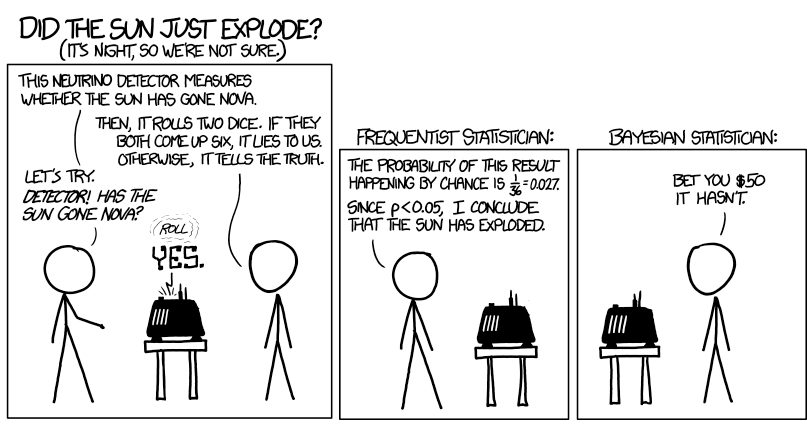
\includegraphics[scale=0.44]{figs/frequentists_vs_bayesians_landscape.png}
    \end{figure}
\end{frame}

\begin{markdown}

### Frequentist inference

Under the frequentist interpretation of probability, the parameters of the population are fixed quantities to be estimated.
\pause\newline

The frequentist is therefore prohibited from making *probabilistic* statements about parameters and hypotheses.
\pause\newline

Probabilities and uncertainties can only be expressed in terms of *repeated sampling* from some target population.

\end{frame}

### Null hypothesis significance testing

Common practice "null hypothesis significance test" (NHST) inference:
\pause

1. Define your experiment, along with the relevant **null** ($H\_0$) and **alternative** ($H_A$) hypotheses, and collect your data.
\pause\newline

3. Compute the relevant *test statistic* $\tilde{z}$ for your null hypothesis.
\pause\newline

4. Compute the $p$-value $p = P(\tilde{z}|H_0)$, i.e. the probability of the observed test statistic under the null distribution.
\pause\newline

5. Reject $H_0$ if $p < \alpha$ where $\alpha$ is an arbitrary significance threshold.

\end{frame}

### Problems with NHST

There are several problems with this procedure.
\pause\newline

1. The $p$-value, $p=P(\tilde{z}|H_0)$, is misleading.
\pause

- It is **not** the probability of the null hypothesis being "true"; this would be $P(H_0|\mathcal{D})$
\pause
- It is **not** the probability that your data was produced by "random chance".
\pause
- It does **not** imply anything about the size of the effect!
\pause
- It says **absolutely nothing** about the alternative hypothesis, $H_A$.

\end{frame}

### Problems with NHST

2. The null hypothesis is almost never true.
\pause\newline

- When is the "true" linear relationship between two values ever *exactly* zero?
\pause\newline

- When is the "true" difference between means every *exactly* zero?
\pause\newline

- What is the point of falsifying something that we know *a priori* must be false?

\end{frame}

% ### Problems with NHST

% 3. The alternative hypothesis is never actually evaluated.
% \pause\newline

% - The null hypothesis is not interesting.
% \pause\newline

% - We care more about $H_A$.
% \pause\newline

% - So why is this never actually evaluated?

% \end{frame}

### Problems with NHST

3. Inference based on a test statistic $\tilde{z}$ is inference based on **hypothetical data** that was never observed.

- The null distribution $P(\tilde{z}|H_0)$ represents an **assumed distribution over data**, not over the hypothesis itself.
\pause\newline

- The $p$-value is the probability of observing your data or something "more extreme" under this distribution.
\pause\newline

- Inference based on this probability implicitly conditions on hypothetical data that was never observed!

\end{frame}

### Problems with NHST

4. Pre-defined hypothesis test procedures often make a wide range of assumptions about the data.
\pause

#### Student's t-test assumptions

- The sample mean is normally distributed.
- The sample variance is $\chi^2$ distributed (or the samples are normally distributed).
- The sample mean and sample variance are independent.
- The variances of both populations are equal (relaxed for Welch's t-test).

---

\end{frame}

### Problems with NHST

5. Uncertainties expressed in the limit of infinite samples are often not helpful.
\pause

- We never have infinite data.
\pause\newline

- In many areas of study such as geoscience, we have very little control over the data generating process.
\pause\newline

% - Data should be used to validate our hypotheses about how complex systems functions.
% \pause\newline

- Uncertainty should be quantified in terms of how well our hypotheses fit the data we have 
and not against hypothetical data that was never observed (see The Likelihood Principle).

\end{frame}

### Problems with NHST

These criticisms are not new...

- Berkson J. **Some difficulties of interpretation encountered in the application of the chi-square test.** Journal of the American Statistical Association. 1938.

- Rozeboom WW. **The fallacy of the null-hypothesis significance test.** Psychological bulletin. 1960.

- Berger JO, Sellke T. **Testing a point null hypothesis: The irreconcilability of p values and evidence.** Journal of the American statistical Association. 1987.

- Johnson DH. **The insignificance of statistical significance testing.** The journal of wildlife management. 1999.

\end{frame}

### Problems with NHST

...and have only continued over time:

- Wasserstein RL, Schirm AL, Lazar NA. **Moving to a world beyond “p< 0.05”**. 2019.

- Amrhein V, Greenland S, McShane B. **Scientists rise up against statistical significance.** Nature. 2019 Mar;567(7748):305-7.

- Gelman A, Stern H. **The difference between “significant” and “not significant” is not itself statistically significant.** The American Statistician. 2006 Nov 1;60(4):328-31.

% - McShane BB, Gal D, Gelman A, Robert C, Tackett JL. Abandon statistical significance. The American Statistician. 2019 Mar 29;73(sup1):235-45.

- Vasishth S, Mertzen D, Jäger LA, Gelman A. **The statistical significance filter leads to overoptimistic expectations of replicability.** Journal of Memory and Language. 2018 Dec 1;103:151-75.

\end{frame}

### What about confidence intervals?

Confidence intervals are generally preferable to p-values.
\pause

However, they are still easy to misinterpret:

1. A particular 95\% confidence interval does not have a 95\% probability of containing the true parameter value.

2. Smaller confidence intervals do not imply "more precise" results.

3. Confidence intervals do not correspond to plausible or likely parameter values.

\pause

Just like p-values, CIs represent **pre-observational probabilities** over the sampling procedure itself.

\end{frame}

### This is confusing...
- Interpreting p-values and confidence intervals is highly counter-intuitive.
\pause\newline

- "Significance" testing forces researchers to make arbitrary "decisions" about their data that are not necessary.
\pause\newline

- The basic theory of random sampling and relative frequency are deceptively intuitive...
\pause\newline

- ...but using the corresponding procedures to answer common research questions is actually not!

\end{frame}


### When to still be frequentist

- Equivalent to the Bayesian solution (e.g. basic linear regression)
\pause\newline
- No prior information is available (rarely the case)
\pause\newline
- Repeated (random) sampling is built into the problem
\pause\newline
- Sampling distribution and experimental design are well controlled
\pause\newline
- Nonparametrics (e.g. bootstrapping) for large, high-dimensional datasets

\end{frame}

### Recommendations
- **Do not** equate "statistical significance" with *scientific significance*.
\pause
- **Do not** selectively show results based on $p$-values or confidence intervals.
\pause
- **Do not** highlight certain results as "statistically significant" based on their $p$-values or confidence intervals.
\pause
- **Avoid** NHST in favor of either the more rigorous Neyman-Pearson theory or a Bayesian approach.

\end{frame}

### Recommendations
- **Do** be careful and conservative with your interpretation of $p$-values and confidence intervals.
\pause
- **Do** be as transparent as possible when reporting statistical results.
\pause
- **Do** prefer problem-specific error metrics and goodness of fit measures like $R^2$ to $p$-values.
\pause
- **Do** use resampling or out-of-sample testing to assess robustness of your results.

\end{frame}

### When to be Bayesian

- Primary goal is to make inferences under uncertainty
\pause\newline
- Small, sparse, or partial data
\pause\newline
- Valuable prior information is available
\pause\newline
- Uncertainty quantification in non-standard models
\pause\newline

In general, it's good to be Bayesian by default :)

\end{frame}

### Bayes rule

We can prove Bayes rule in just three lines!
\pause
    
$$ p(A,B) = p(B,A) $$
\pause
    
$$ p(A|B)P(B) = p(B|A)p(A) $$
\pause
 
$$ p(A|B) = \frac{p(B|A)p(A)}{p(B)} $$
    
\end{frame}

% \begin{frame}{Statistical inference via Bayes rule}
%     Let $\theta$ represent some parameter of interest for a dataset $\mathcal{D}$. Then by Bayes rule:
%     $$
%     p(\theta | \mathcal{D}) = \frac{p(\mathcal{D} | \theta)p(\theta)}{p(\mathcal{D})}
%     $$
%     \pause
    
%     $P(\theta | \mathcal{D})$ is called the \textbf{posterior} distribution over parameters $\theta$.
%     \pause\newline
    
%     $P(\mathcal{D} | \theta)$ is called the \textbf{likelihood} and is a function of $\theta$.
%     \pause\newline
    
%     $P(\theta)$ is called the \textbf{prior} distribution over $\theta$.
%     \pause\newline

%     $P(\mathcal{D})$ is called the \textbf{marginal likelihood} or \textbf{evidence}.
% \end{frame}

% \begin{frame}{Statistical inference via Bayes rule}
%     We can also write the marginal likelihood as:
    
%     $$p(\mathcal{D}) = \int_{\theta} p(\mathcal{D}|\theta)p(\theta)d\theta= \mathbb{E}_{\theta}[p(\mathcal{D}|\theta)]$$
%     \pause\newline
    
%     Thus, the marginal is the \textbf{expectation} of the likelihood.
% \end{frame}

% Apparently it's possible to use Markdown via the markdown package. I'm gonna do that now!

%%begin novalidate

### Statistical inference via Bayes rule

Let $A = \theta$ be our unobserved variables of interest and $B = \mathcal{D}$ be our observed data.
\pause\newline

The posterior distribution $p(\theta | \mathcal{D})$ represents our belief or knowledge of $\theta$ after the data has been taken into account.
\pause\newline

$\theta$ can be as simple as a mean or proportion...
\pause\newline

...or it can be an arbitrarily large set of parameters for a complex model.

\end{frame}

### Statistical inference via Bayes rule

Once we have a summary of $P(\theta | \mathcal{D})$, we can ask questions like:
\newline

What is the probability that $\mu > 0$?
\newline

What is the probability that $\mu\_1 > \mu_2$ for groups 1 and 2?
\newline

What is the probability that the slope of a linear regression $\beta > 0$?

\end{frame}

% ### Maximum likelihood estimation (MLE)

% Have you ever fitted an OLS line or optimized the mean squared error?
% \pause\newline

% Then congratulations, you're familiar with MLE!
% \pause\newline

% MLE aims to maximize the **likelihood function** $P(\mathcal{D}|\theta)$ w.r.t $\theta$.
% \pause\newline

% Typically, this is done via the **negative log likelihood**:
% $$
% \mathcal{L}(\theta) = -\log P(\mathcal{D}|\theta)
% $$

% and solving $\frac{\partial \mathcal{L}}{\partial \theta} = 0$ for $\theta$.

% \end{frame}

% ### Maximum likelihood estimation (MLE)

% Common loss functions you may have used:

% - Mean squared error, $\frac{1}{N}\sum\_{i=1}^N (\hat{y}\_i - y\_i)^2$
% \pause\newline
% - Mean absolute error, $\frac{1}{N}\sum\_{i=1}^N |\hat{y}\_i - y\_i|$
% \pause\newline
% - Cross entropy, $-\frac{1}{N}\sum\_{i=1}^N y\_i\log \hat{y\_i} + (1-y\_i)\log(1-\hat{y}\_i)$
% \pause\newline

% All are forms of maximum likelihood.

% \end{frame}

### Maximum a posteriori (MAP) estimation

Recall Bayes rule:

$$
P(\theta | \mathcal{D}) = \frac{P(\mathcal{D} | \theta)P(\theta)}{P(\mathcal{D})}
$$
\pause

**Maximum a posteriori** (MAP) estimation maximizes $P(\theta | \mathcal{D}) \propto P(\mathcal{D} | \theta)P(\theta)$ w.r.t $\theta$.
\pause

Or equivalently, minimizes:
$$
\mathcal{L}_{\mathcal{D}}(\theta) = -\log P(\mathcal{D}|\theta) - \log P(\theta)
$$
\pause
Notice that maximum likelihood estimation (MLE) is just a special case of MAP.

\end{frame}

### Estimating the posterior distribution

MAP provides a point estimate of $\theta$.
\pause\newline

As Bayesians, we are interested in estimating the full distribution $P(\theta|\mathcal{D})$.
\pause\newline

Unfortunately, that's pretty hard!
$$
P(\theta | \mathcal{D}) = \frac{P(\mathcal{D} | \theta)P(\theta)}{\int\_\theta P(\mathcal{D}|\theta)P(\theta)d\theta}
$$

The integral on the bottom is typically intractable for non-trivial models.

\end{frame}

### Markov Chain Monte Carlo

Enter... Markov Chain Monte Carlo! (MCMC)
\pause\newline

Basic idea: Sample numerically via a **random walk** in the space of $\theta$.
\pause\newline

In the limit of infinite steps, the path of the walk will follow $P(\theta|\mathcal{D})$.
\pause\newline

Unfortunately, this is often quite inefficient.
\pause\newline

Modern state-of-the-art samplers are typically variants \textbf{Hamiltonian Monte Carlo} (HMC) which require gradients.

\end{frame}

% ### Markov Chain Monte Carlo

% Let $f(\theta) = P(\mathcal{D}|\theta)P(\theta)$
% \pause\newline

% 1. Choose some starting point $\theta\_0$.
% \pause\newline
% 2. Sample a new *proposed* point $\theta^*$ from a **proposal distribution**.
% \pause\newline
% 3. If $f({\theta}^* ) > f(\theta\_0)$, accept $\theta^*$ as the new starting point.
% \pause\newline
% 4. Otherwise, accept with probability $\frac{f(\theta^*)}{f(\theta\_0)}$ or reject the proposed sample.

% \end{frame}

### Hamiltonian Monte Carlo

\begin{figure}
    \centering
    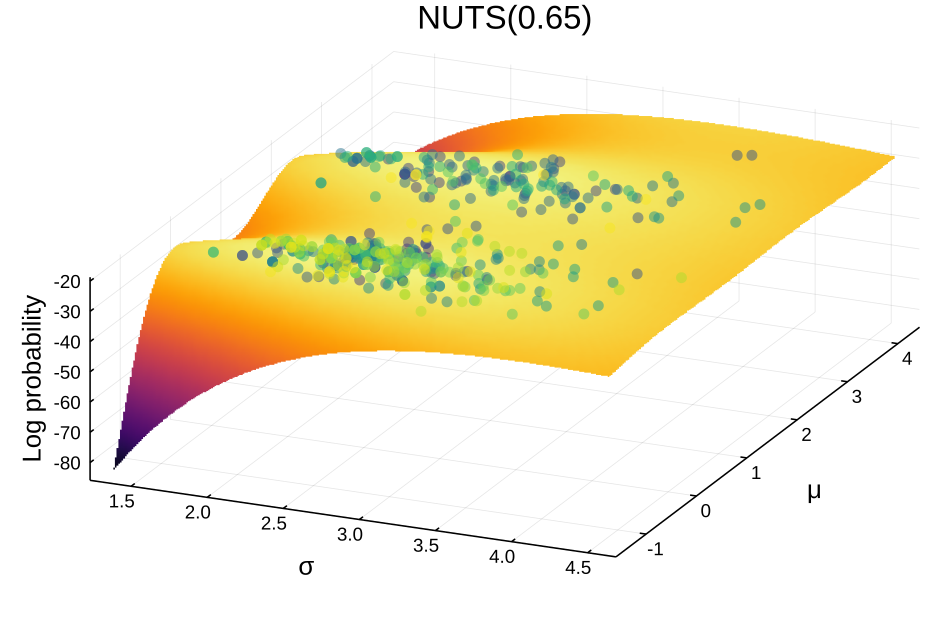
\includegraphics[scale=0.55]{figs/sampler-viz-nuts.png}
    \caption{NUTS sampler visualization (source: Turing.jl documentation)}
\end{figure}

\end{frame}

### Interpreting the output

The output of MCMC and HMC algorithms is sequence of samples, typically referred to as a **chain** or a **trace**.
\pause

\begin{figure}
    \centering
    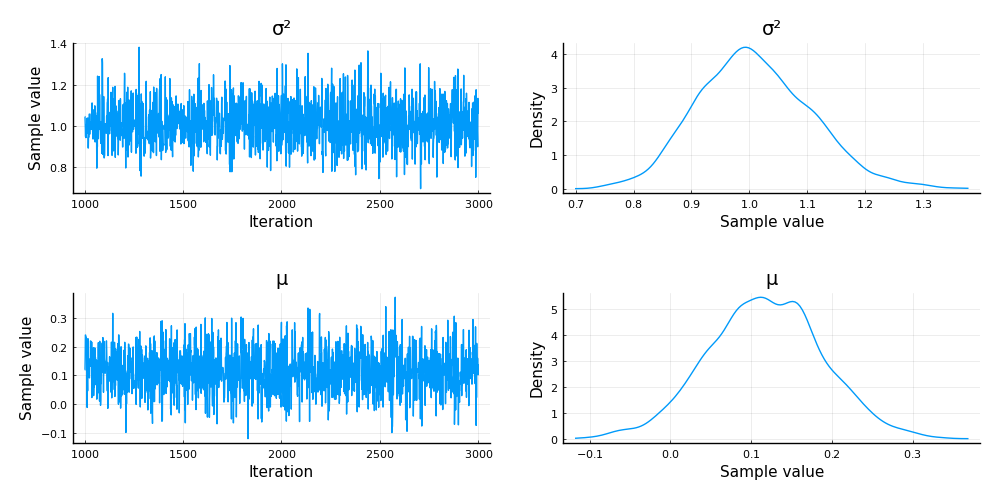
\includegraphics[scale=0.45]{figs/simple_chain.png}
\end{figure}

\end{frame}

\end{markdown}

\begin{frame}{Overview of algorithms for Bayesian inference}
    \begin{table}[]
        \centering
        \begin{tabular}{|p{3em}|p{5em}|p{5em}|p{6em}|p{6em}|}
            \hline
              & Forward runs & Gradients required? & Parallelizable? & Asymptotic convergence \\
             \hline
             MCMC & \numrange{e4}{e6} & No & No & Yes \\
             HMC & \numrange{e3}{e5} & Yes & No & Yes \\
             VI & \numrange{e2}{e4} & Yes & Batch & No \\
             SMC & \numrange{e3}{e5} & No & Yes & Yes \\
             EKS & \numrange{e3}{e4} & No & Yes & Gaussian \\
             IS & \numrange{e1}{e3} & No & Yes & No \\
             \hline
        \end{tabular}
        \label{tab:inference_algs}
    \end{table}
\end{frame}

\begin{markdown}

### Limitations and challenges
Bayesian inference provides a flexible and intuitive framework for data analysis and generative modeling... **but**
\pause

- Choosing good priors can be difficult.
\pause\newline
- MCMC is computationally expensive, especially with large numbers of parameters.
\pause\newline
- Practical analysis of the inference results can be time consuming.
\pause\newline
- Software support is not as comprehensive as for ``classical'' frequentist analyses.

\end{frame}

### Coming up next...
- Probabilistic programming
\pause\newline
- Bayesian generalized linear models
\pause\newline
- Model diagnostics and criticism
\pause\newline
- Example application to observational data from the Arctic

\end{frame}

\end{markdown}

\section{Part II: Bayes by example}

\begin{frame}{Follow along!}

Part II of the workshop consists of a series of Jupyter notebooks.
\newline

\begin{figure}
\centering

\includegraphics[width=0.25\textwidth]{figs/bayes_workshop_qr.png}
\end{figure}

You can directly open these notebooks on Google Colab if you do not want to bother setting up a new python environment!

\end{frame}

%%%%%%%%%%%%%%%%%%%%%%

%%novalidate

% \section{Conclusion}

% ### Important topics not covered

% - Model comparison (e.g. via Bayes factors)
% \pause\newline
% - Model criticism and debugging
% \pause\newline
% - Time series/stochastic processes
% \pause\newline
% - Hierarchical models
% \pause

% Maybe next time? :)

% \end{frame}

% \begin{frame}{A brief review of probability theory}

%     \tikz[remember picture, overlay] \node[anchor=west] at ($(current page.center)-(0.65,-0.5)$) {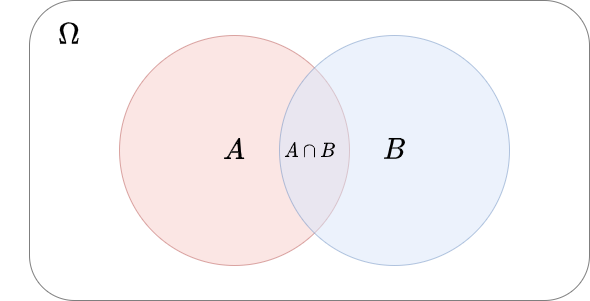
\includegraphics[scale=0.38]{figs/prob_events.png}};

%     $ (\Omega,\mathcal{F},P) $ defines a \textbf{probability space}.
%     \pause\newline

%     $\Omega$ is the \textbf{sample space}.
%     \pause\newline
    
%     $\mathcal{F}$ is the \textbf{event space}.
%     \pause\newline
    
%     $P$ is the \textbf{probability function} which assigns probabilities in $[0,1]$ to events in $\mathcal{F}$.
    
% \end{frame}

% \begin{frame}{A brief review of probability theory}
%     \textbf{Multiplication rule}

%     $ P(A\cap B) = P(A,B) = P(A|B)P(B) $
%     \pause\newline
    
%     \textbf{Addition rule}
    
%     $ P(A\cup B) = P(A+B) = P(A) + P(B) - P(A\cap B) $
%     \pause\newline
    
%     \textbf{Independence}
    
%     $ P(A | B) = P(A)$ if and only if $A$ and $B$ are \textbf{independent}.
    
%     $ P(A | B) = P(A) \leftrightarrow P(A,B) = P(A)P(B)$
% \end{frame}

% \begin{frame}{A brief review of probability theory}
%     \textbf{Law of total probability}

%     $P(A) = P(A|B)P(B) + P(A|\neg B)P(\neg B)$
%     \pause\newline
    
%     \textbf{The chain rule of probability}

%     $P(A,B,C) = P(A|B,C)P(B|C)P(C)$
%     \pause
    
%     or more generally:
    
%     $P(X_1,\dots,X_k) = P(X_1)\prod_{i=2}^{k} P(X_{i}|X_{i-1},\dots,X_1)$
% \end{frame}

% \begin{frame}{Random variables}
%     A \textbf{random variable} (RV) is a function $\mathcal{X}: \Omega \rightarrow E$, where $\Omega$ is the \textbf{sample space} and $E$ is a \textbf{measureable quantity} of interest.
%     \pause\newline
    
%     For \textbf{continuous} random variables, $E\subseteq \mathbb{R}$.
%     \pause\newline
    
%     For \textbf{discrete numerical} random variables, $E\subseteq \mathbb{Z}$.
%     \pause\newline
    
%     For \textbf{discrete binary} (or "indicator") random variables, $|E| = 2$, e.g. $\{0,1\}$.
%     \pause\newline
    
%     For \textbf{discrete categorical} random variables, $|E| = k$, where $k$ is the number of groups/categories.
% \end{frame}

% \begin{frame}{Probability densities and expectation}
% For discrete RVs, the \textbf{probability mass function} (PMF) is defined as:

% $$\pi: \mathcal{X} \rightarrow [0,1], \sum_{x \in \mathcal{X}} \pi(x) = 1$$

% and the \textbf{expected value} (or \textbf{expectation}) is:

% $$\mathbb{E}[\mathcal{X}] = \sum_{x \in \mathcal{X}} x\pi(x)$$
% \end{frame}

% \begin{frame}{Probability densities and expectation}
%     For continuous random variables, the \textbf{probability density function} (PDF) is defined as:
    
%     $$\pi: \mathcal{X} \rightarrow [0,1], \int_{x \in \mathcal{X}} \pi(x)dx = 1$$
    
%     and similarly, the expectation is:
    
%     $$\mathbb{E}[\mathcal{X}] = \int_{x \in \mathcal{X}} x\pi(x)dx$$
% \end{frame}

% \begin{frame}{Probability densities and expectation}
%     Note that it is common to write $p(\mathcal{X})$ or $p(x)$ where $x \in E$.
%     \pause\newline
    
%     This is a slight abuse of notation.
%     \newline
    
%     $p(\mathcal{X})$ typically refers to the density function, $p(x) = \pi$.
%     \pause\newline
    
%     $p(x)$ is the density evaluated at $x$, i.e. $\pi(x)$.
% \end{frame}

\end{document}
